\LARGE{ \textbf {Лекция №7}}\\
\Large{ \textbf {Асинхронный RS-триггер}}\\
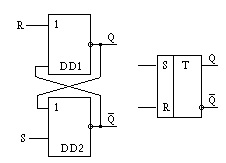
\includegraphics[width=\linewidth/2]{21} \\
Данный триггер реализованый в базисе ИЛИ-НЕ является триггером с прямыми входами.
\textbf {Прямые входы} означают, что активным уровнем управляющих сигналов является уровень логической единицы.
В силу двойственности алгебры логики аналогичный триггер можео реализовать в базисе И-НЕ.
Из формул 1 и 2 данного параграфа можно получить формулы для И-НЕ.\\
$Q_n+1 =\overline{ \overline{S_n} \cdot \overline{( \overline{R_n} Q_n })}$\\
$\overline{Q_{n+1} }= \overline{  \overline{R_n} + \overline{ \overline{S_n} Q_n }}$



\textbf {Асинхронный RS-триггер И-НЕ}\\
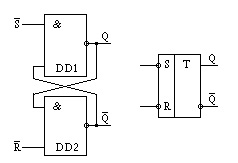
\includegraphics[width=\linewidth/2]{22} \\

Активным переключающим сигналом является урованеь логического 0.\\
$\overline{S} = 0,1,0,1$\\
$\overline{R} = 0,0,1,1$\\
Хранение, установка 1, установка 0, запрещен.\\

\newpage
Временные диаграмы работы асинхронного RS-триггера в базисе И-НЕ.

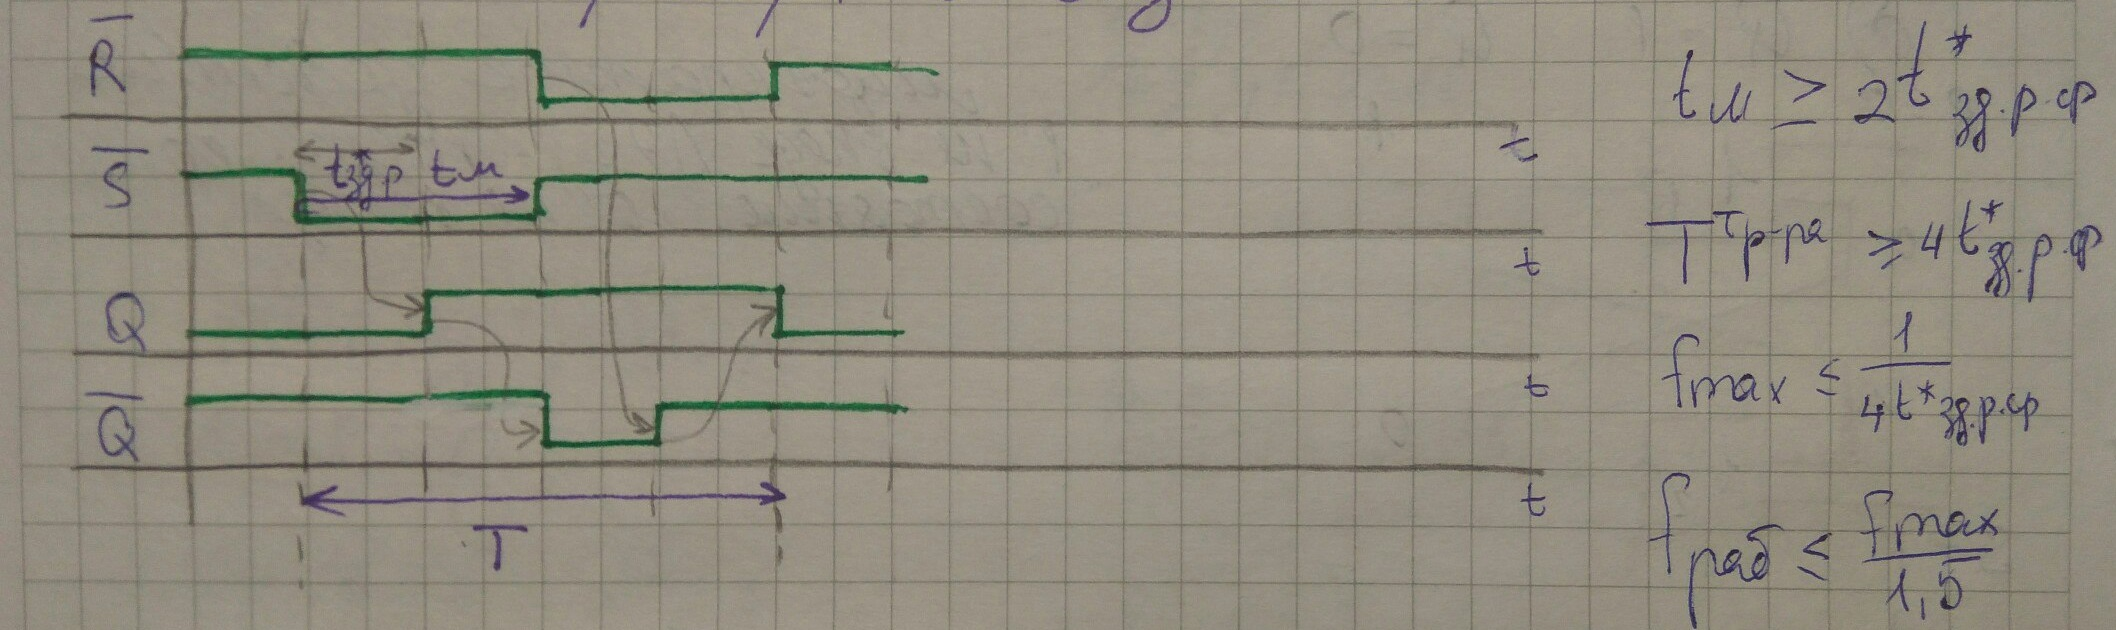
\includegraphics[width=\linewidth]{29}\\


Будем считать, что триггер в начальный момент времени\\
$t_{zader} => 2t^*_{zaderSR}$\\
$T^{triger} => 4 t^*_{zaderSR}$ \\

Состязания в асинхронных схемах (гонки сигналов).\\

Логические функции описывают лог схемы идеализированно, так как не учитывают задержки на логических элементах.\\
Наличие задержек приводит к появлению состязаний сигналов.\\
$F = \overline{A \cdot A} = \overline{0} = 1 $\\ \\
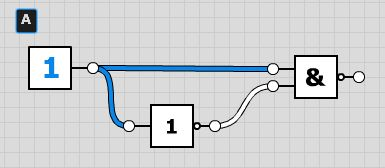
\includegraphics[width=\linewidth/2]{15}\\
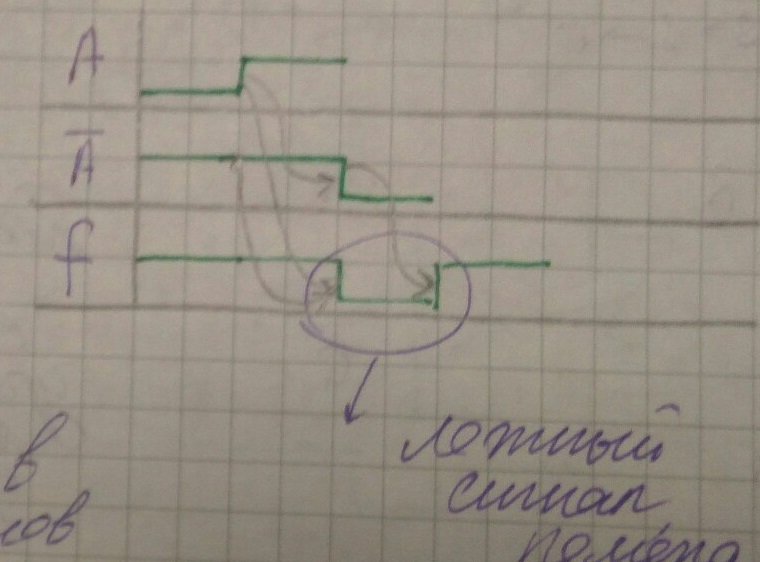
\includegraphics[width=\linewidth/2]{30}\\

Из-за задержки возникают ложные сигналы(помехи) в момент переключения значения А.\\
Возможность появления помехи в результате гонки сигналов называют статическим риском сбоя.\\
Для исключения таких сбоев вводят стробирование.\\
\textbf {Стробирование} -  выделение из информационного сигнала части свободной от ложных сигналов.\\
Процесс стробирования переодическими сигналами \textbf {называются синхронизацией},
а период следования синхросигналов \textbf {тактом}. \\

В схемотехнике чаще всего комбинационная схема заканичивается триггером, поэтому стробирование вводят на входах триггерных схем.\\
В общем случае - вводятся в последнем каскаде.

Триггеры, информационные сигналы которых стробируются специальными
переодическими сигналами навзываются \textbf {синхронными триггерами}.\\
Кроме исключения ложных сигналов синхронизация создает условие для одновременного изменения состояния входов триггеров,
то есть так называемая синхронная работа.

\newpage
\textbf {Синхронные триггеры.}\\
Синхронные триггеры имеют один или несколько входов синхронизации. Обозначаются C. \\
Сигнал синхронизации разрешает прием сигналов с информационных входов. \\
Если вход С прямой , то при С=0 обрабатывать сигналы запрещено.\\
\textbf {Синхронный RS-триггер. И-НЕ}\\
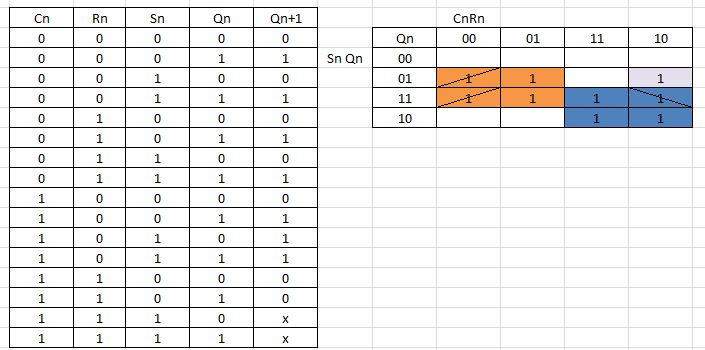
\includegraphics[width=\linewidth*3/4]{23}\\
$Q_{n+1} = \overline{C_n}Q_n + C_n \cdot S_n + \overline{R_n} \cdot Q_n $\\
\qquad $  = Q_n \cdot (\overline{C_n} + \overline{R_n} ) + C_n \cdot S_n$\\
$ = C_n S_n + \overline{C_n R_n} \cdot Q_n$\\
$\overline{Q_{n+1}} = C_n R_n + \overline{C_n S_n} \cdot \overline{Q_n}$\\
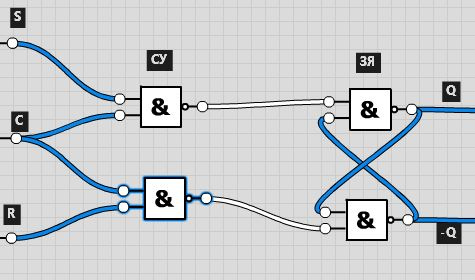
\includegraphics[width=\linewidth*2/3]{16}\\
\newpage
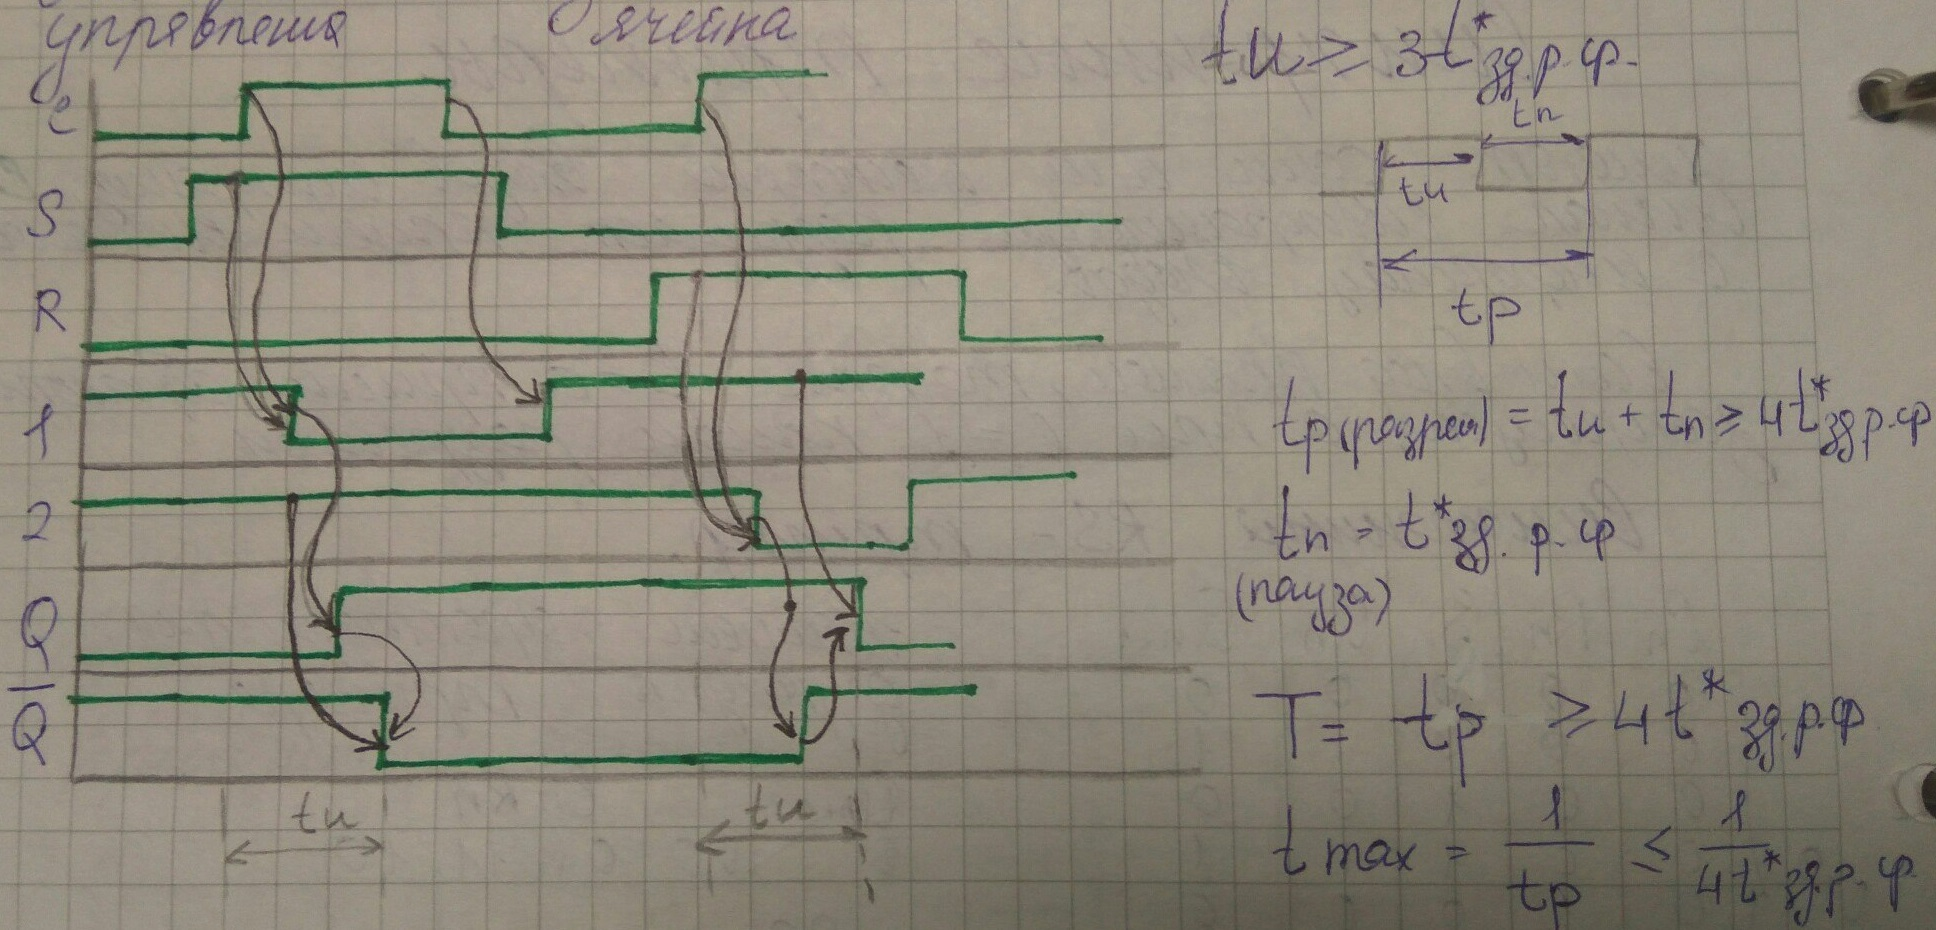
\includegraphics[width=\linewidth]{31}\\

$t_{u} => 3t^*_{zaderSR}$\\
$t_{p} => t_u + t_n $\\
$t_{n} => t^*_{zaderSR}$\\
$T = t_p => 4t^*_{zaderSR} $\\
$t_{max} = \frac{1}{t_p} <= \frac{1}{ 4t^*_{zaderSR}} $\\
Синхронный RS-триггер. ИЛИ-НЕ. \\
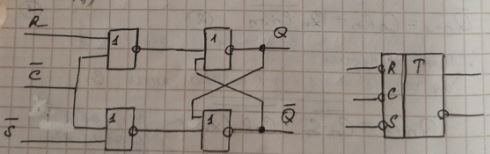
\includegraphics[width=\linewidth*2/3]{24}\\



\textbf {Синхронный D-триггер.}\\
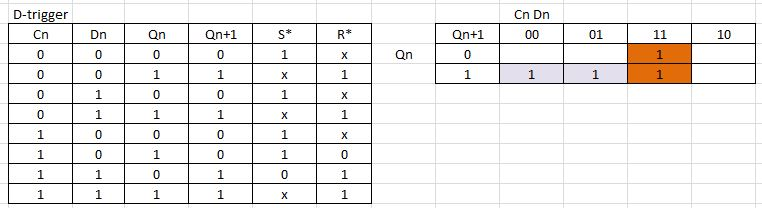
\includegraphics[width=\linewidth*3/4]{25}\\
$Q_{n+1} = \overline{C_n} \cdot Q_n + C_n \cdot D_n $\\
$C = 1  -> Q_{n+1} - D_n $\\


Это просто повторитель, а не запоминающая ячейка.\\
$S* = f(C_n, D_n,Q_n) $\\
$R* = p(C_n, D_n,Q_n) $\\
$S* = \overline{C_n} \overline{D_n} = \overline{C_n \cdot D_n} $\\
$R* = \overline{C_n} D_n = \overline{C_n \cdot \overline{D_n}} $\\
В данном виде требуется "лишний инвертор", надо от него избавить.\\
$R* = \overline{C_n} D_n = D_n(\overline{C_n} + \overline{C_n}) + \overline{C_n} = $\\
$D_n C_n  + D_n \overline{ C_n} + \overline{C_n} = $\\
$ D_n C_n  + \overline{C_n}(D_n + 1) = $\\
$D_n C_n + \overline{C_n}  $\\
$\overline{S^*}  + \overline{C_n}$ \\
$ \overline{S^* \cdot C_n}$\\
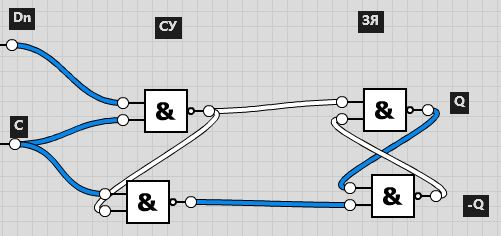
\includegraphics[width=\linewidth]{17}

DV(E) - trigger\\
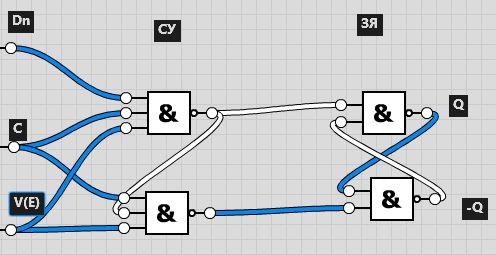
\includegraphics[width=\linewidth]{18}

Логические уравнения синхронного Д-триггера могут быть полученыил лог уравнений RS-триггера путем замены S на D, R на $\overline{D}$.\\
\newpage
\textbf {Асинхронный Т-триггер или счетный триггер.}\\
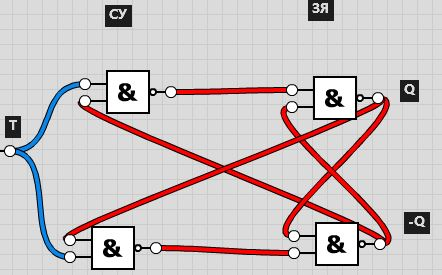
\includegraphics[width=\linewidth*3/4]{19}

По опредению он функционирует с одной таблицей перехода. \\
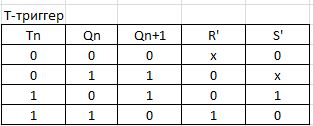
\includegraphics[width=\linewidth/2]{26}

Триггер переключается в противоположное состояние при подаче импульса на Т.\\
$Q_{n+1} = \overline{T_n} \cdot Q_n + \overline{Q_n} + T_n = T_n +M2 Q_n $\\
$\overline{R`} = \overline{T_n} \cdot Q_n$\\
$\overline{S`} = \overline{T_n} \cdot Q_n$\\
\newpage
Значения сигналов не совпадают с Д-триггером, здесь R,S не инверсные.
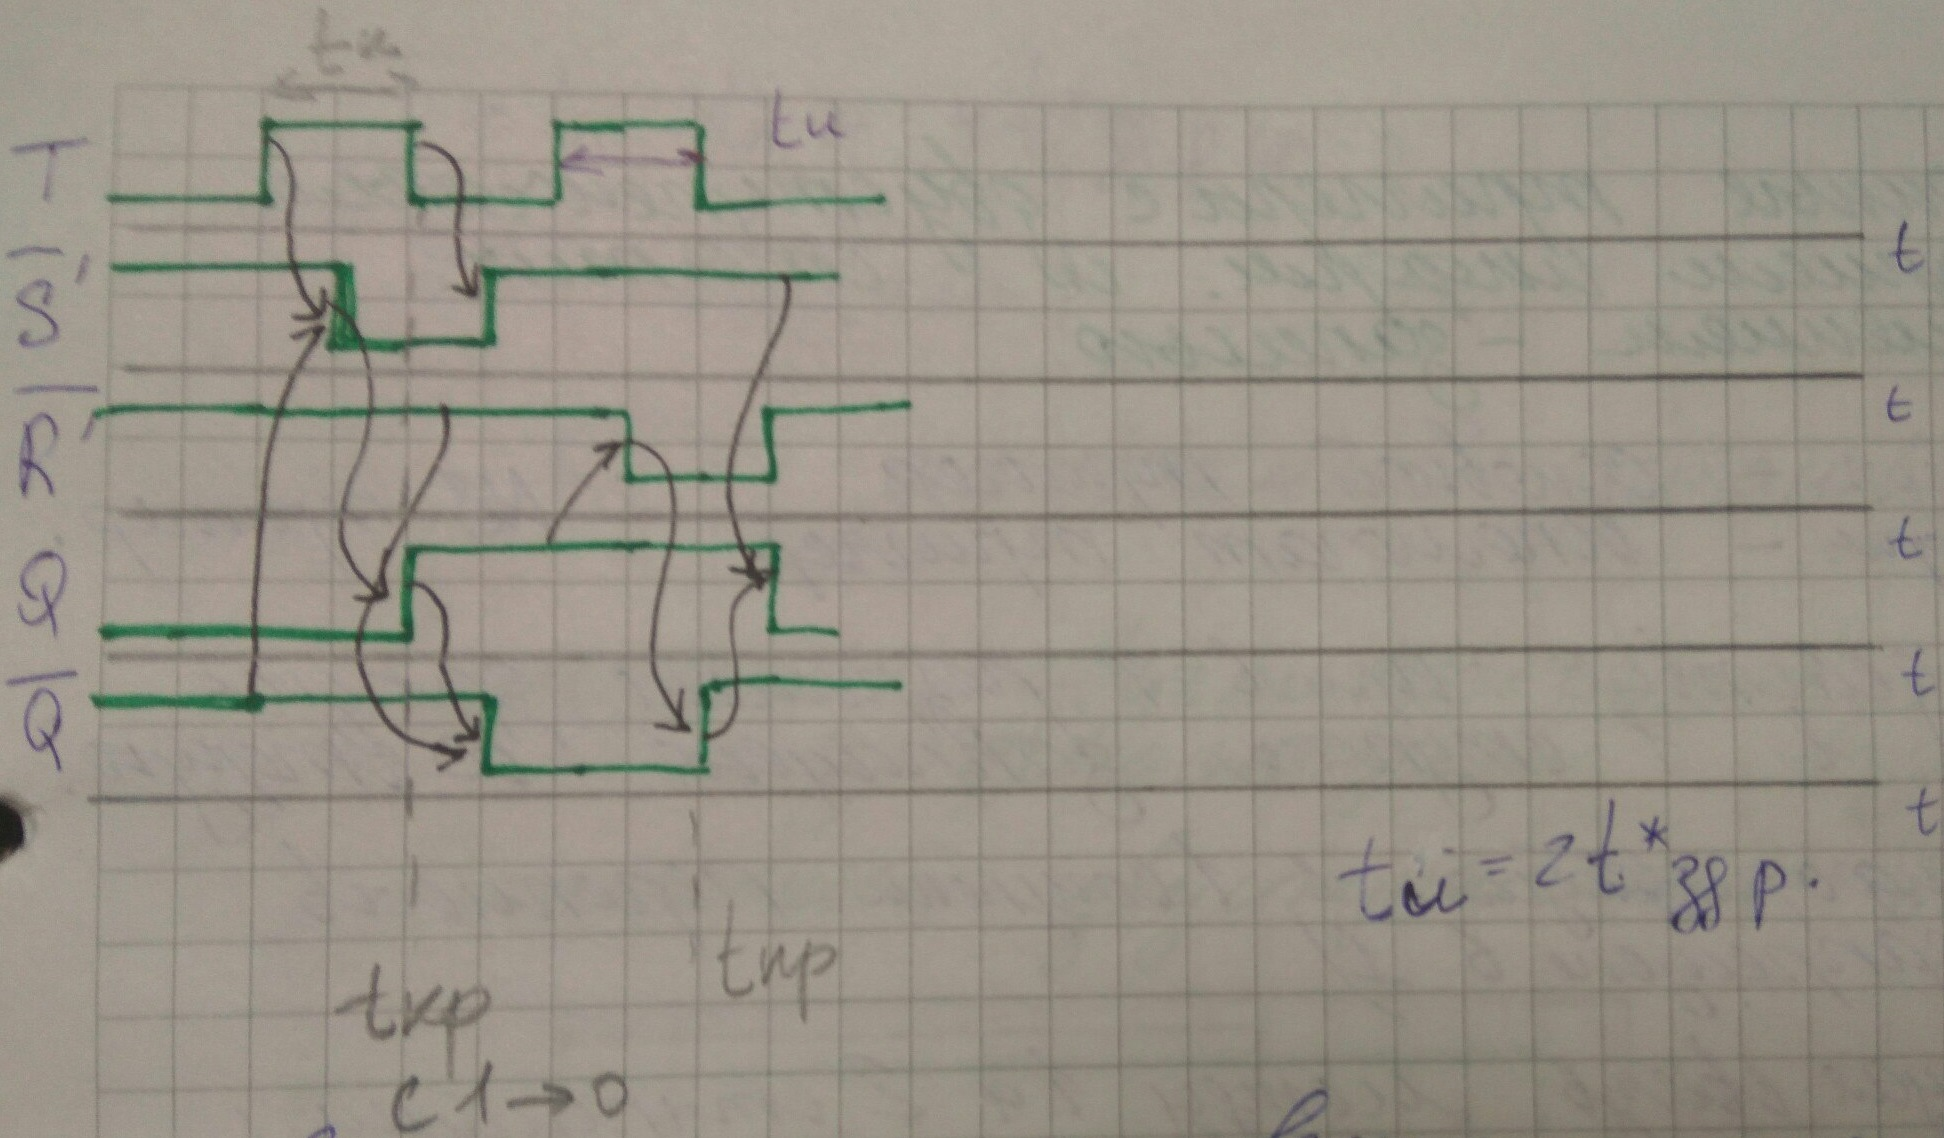
\includegraphics[width=\linewidth]{32}\\

$t_{u} => 2t^*_{zaderSR}$\\

Если длительность входного сигнала больше длительности переходных процессов в триггере, то в сземе возникают автоколебания.
Так как при действии одного сигнала Т триггер многократно переключить в 0 и обратно.
Генерация возникает, если время импульса будет больше, чем $2t^*$.
Если же время импулься будет меньше $2t^*$, то триггер не переключиться вообще.\\
Схема работоспособна когда время импульса строго равно  $2t^*$.\\
Во-вторых никому не нужна схема, работающая на одной частоте.\\


Из-за этих недостатков необходимо ввести задержку между лог элементами 1 и 3 , 2 и 4. \\
Точно таким же недостатком обладают ЖК-триггеры. \\
Поэтому счетные триггеры и жк триггеры реализуются, как двухступеньчатые триггеры реализуются, как двуступеньчатые триггеры или
как триггеры с динамическим управлением запиью.
